\section{Interested Parties}
In this section we will be taking a look at some potentially interested parties, in order to determine the extent of their interest in solving the problem along with the extent of their influence on the matter.

\subsection{Employees}
%The employees, understandably, have a great interest in the work schedule. It affects both their job and personal life, since they (probably - PERHAPS SOURCE) have to make plans around their work, so most of their time is based around their work schedule.

One of the most important interested parties are the employees since they can experience significant health and social issues if their schedule is poorly constructed. Research shows that the risk of getting chronic health conditions is increased by having long and/or rotating shifts and poor work scheduling \parencite{mchugh_qualitative_2020}. Less deadly, but still important, issues following poor work scheduling include limited time with family and less social life, which can lead to stress \parencite{stephanie_willett_7_2019}. Therefore, it seems obvious that employees would consider proper work scheduling to be a top priority, hence the focus of our project.

These problems do not only impact the employees themselves, but their families as well. According to a statistic gathered by the law firm Lund Bennet \parencite{lund_bennet_rise_2017-1}, shift workers are more likely to get divorced, due to the unpredictability of their shifts and potential night shifts, especially if both partners are working shifts there is a particularly high divorce rate. There are therefore multiple parties who have an interest in solving or preventing the problem of bad scheduling.

Conflicts of interest may occur between employers and employees. It is of course also very important to remember that the satisfaction of the employees is not necessarily an obstacle or a problem for the employers. Since proper work scheduling could potentially reduce the number of sick days and stress, the company would most likely see some benefit from this. Furthermore, satisfied employees are more likely to not switch jobs. This will of course be of benefit to the company since they can spend less resources on recruiting and training new employees. \parencite{daniel_sgroi_happiness_nodate}

Although the employees have a great interest in the schedule, their influence is not that significant, since it is the employers that are responsible for creating the schedule. The other employees are able to express requests that the employers have to have in mind, \parencite{industriens_overenskomst} but in the end, the average employees do not have the biggest influence on their work schedule.

Luckily, the employees are usually in a union, that puts demands and limitations on what the employers are allowed to do, regarding the work schedule.  

\subsection{Unions}
As explained above, the union is the party that makes sure an employer does not treat their employee inhuman. They are the ones who bargain a deal of what is allowed to demand between the employer and employee, hence an interest in the work-schedule. Their interest lies in the fact, that the employee is a customer of theirs, and their job is to make sure their customers are treated fairly. That said, their interest is not necessarily on par with the employees, since it does not directly affect the ones who are making the schedule personally. However, they still have a greater influence than the employees since they are the ones responsible for making the agreement.

\subsection{Employers}
The employers are the ones responsible for making sure the schedules are made and ensuring that they meet the requirements of the relevant union agreements. The employer has a vested interest in making sure that the schedule meets the requirements of the union agreement, since a breach thereof can in the worst case lead to the employer being brought to court by the union, or in smaller cases be obliged to pay fees \parencite{overenskomstbrud}. The employer also has an interest in getting the work schedule created as efficiently as possible, as they need to invest time in the creation of the work schedule that  could have been used elsewhere. 

The employers themselves need to be considered when talking about this project. As much as the employer would like to have the worker working every single hour, they are awake, that simply is not humanly possible. It is necessary that a balance between what is expected and what the worker can actually provide is reached. This typically culminates either in what is known as a full-time job, where an employee works for example from 9.am to 5.pm or giving the employee shifts where they have to work. Our project focuses on the second part, the employees that work on varying shifts.  %fixed

\begin{table}[ht!]
    \centering
    \begin{tabular}{lllll}
        \toprule
                  & Team 1  & Team 2  & Team 3  & Team 4  \\
                  \midrule
        Thursday  & 6am-6pm &         & 6pm-6am &         \\
        Friday    &         & 6am-6pm &         & 6pm-6am \\
        Saturday  &         & 6am-6pm &         & 6pm-6am \\
        Sunday    &         &         &         &         \\
        Monday    & 6am-6pm &         & 6pm-6am &         \\
        Tuesday   & 6am-6pm &         & 6pm-6am &         \\
        Wednesday &         & 6am-6pm &         & 6pm-6am \\
        \bottomrule
    \end{tabular}
    \caption{A table showing an example of how a schedule could be set up, with 2 day teams and 2 night teams.}
    \label{tab:exampleSchedule}
\end{table}

As mentioned, the employer would benefit the most from constant production. But since a human cannot work every single hour, another option is needed. Instead of having the same people working all day, there could instead be four teams, two day shift teams and two night shift teams. This could for example be in the pattern seen in Table \ref{tab:exampleSchedule}.

This allows production to be in action 24 hours a day, six days a week, only missing Sunday. There are of course a lot of things that need to be taken into consideration with such a system, primarily the union agreement the workers work under. This includes things like bonuses, when working "bad" hours, such as team three and four, who work night shifts. Nevertheless, there is still a balance with this schedule, allowing the employer to have constant production, and the employees to have time off.

Since the employer is the one making the schedule, they are the ones with the most influence with regards to deciding how it is done. Although, whether the employer has the spare resources to invest will likely vary greatly from one company/organization to another.


\begin{figure}[ht!]
    \centering
    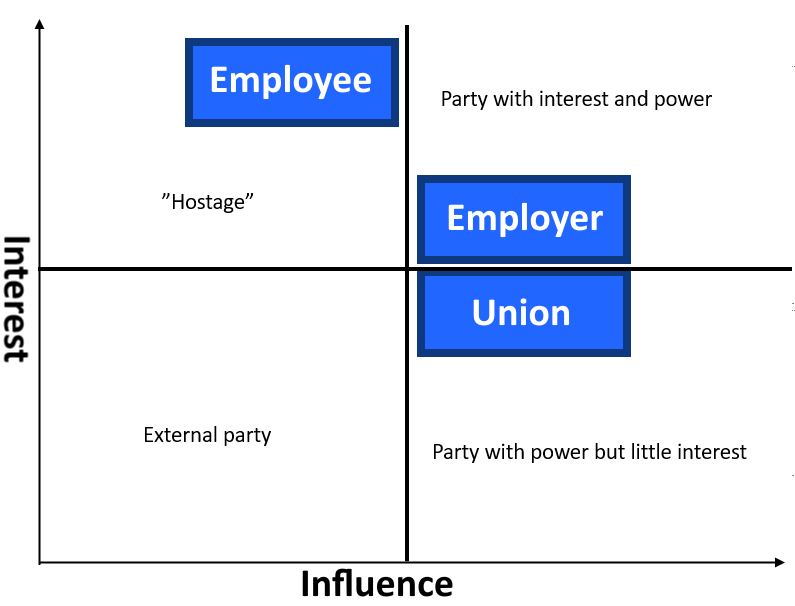
\includegraphics[width=100mm]{media/NewInterestedParties.PNG}
    \caption{Visualization of the interested parties, relative to interest and influence.}
    \label{fig:Interested parties graph}
\end{figure}

As visualized in Figure \ref{fig:Interested parties graph}, the employee is the party with the greatest interest since it affects their lives directly. Although, it is also the party with the least influence, since they do not have the biggest influence in demands and requirements, after all it is the union that is in control of that. Therefore, the employees become more or less of a "hostage" in this situation, since they only have little power when it comes to determining their own work schedule. We have placed the union party and the employer party at the same level of influence, but the employer has a bit more interest than the union. They have the same influence since they are the two parties responsible for making an agreement on how to treat the employees, but the employer has a greater interest since they are affected more directly than the union. The employer is responsible for following the agreement and can face big consequences if the agreement is broken. Beyond that, the employer is making money off the employees, hence a greater interest since it affects their income and therefore their lives.
